\chapter{EAS Selection Efficiency with Increased NSB}\label{Ch:SelectEff}


Selection Efficiency of EAS under increased NSB
\begin{itemize}
\item Smearing real data with extra noise
\item Simulating EAS with an increased NSB
\item Talk about differences in smearing and simulating EAS (different triggering conditions)
\item Energy and Xmas resolution and bias
\item Rp bias
\item differences in track length
\end{itemize}



Typically the NSB measured at PAO is in Units of ADC$^2$. As the signal is AC coupled, this is the variance around the zero and is directly proportional to the fluctuations in the NSB. The average value of the NSB is:
\begin{equation}
\sigma^2 \sim 25 \ \mathrm{ADC}^2
\end{equation}
Converting the variance into photons by using:
\begin{eqnarray}
\sigma^2_{pe} &=& [\sigma^2_{\mathrm{ADC}}]^{\mathrm{sky}} \ / \ \mathrm{A}^2_{\mathrm{G}} \label{eq:simgaPE} \\
\mathrm{n}_{\mathrm{ph}} &=& \frac{\sigma^2_{pe}}{(1 + \mathrm{V}_{\mathrm{G}})} \label{eq:numPhoton}
\end{eqnarray}
where $\sigma_{pe}$ is the standard deviation of the photo-electron count, n$_{\mathrm{ph}}$ is the photon count and A$_{\mathrm{G}}$ is equal to:
\begin{equation}\label{eq:abs_gain}
\mathrm{A}_{\mathrm{G}} = \frac{1}{\mathrm{C}_{\mathrm{FD}}.\mathrm{f}.\mathrm{Q}}
\end{equation}
where
\begin{itemize}
\item[] A$_{\mathrm{G}}$ is the absolute gain (ADC/photo-electron)
\item[] $\mathrm{C}_{\mathrm{FD}}$ is the FD pixel calibration constant.
\item[] Q is the Quantum efficiency of the PMT.
\item[] f is the efficiency if the telescope optics.
\end{itemize}

/*------ Find reference to number below ------*/

Assuming typical measured values for C$_{\mathrm{FD}}$, Q and f shown in:

\begin{center}
\begin{tabular}{|c|c|}
\hline
C$_{\mathrm{FD}}$ & 4.5 photons/ADC \\
\hline
Q & 0.29 \\
\hline
f & 0.465 \\
\hline
\end{tabular}
\end{center}

Therefore can now calculate A$_{\mathrm{G}}$ from Eq. \ref{eq:abs_gain} and using 

\begin{figure}[!hp]
\centering
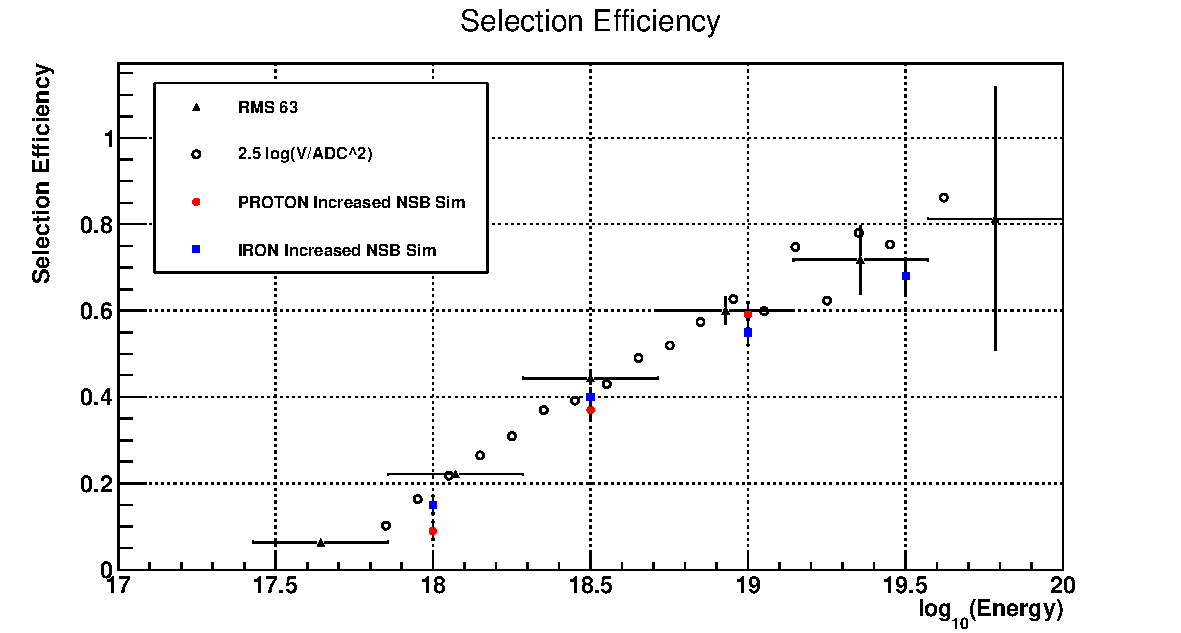
\includegraphics[width=\textwidth]{chapters/graphs/SelectionEff/SelectionEff_errorbars_10timesNSB.pdf}
\caption{Selection Efficiency plot containing data from both the Smearing method and simulated showers. These results are compared to the Work done by M. Unger.}
\end{figure}

\begin{figure}
\centering
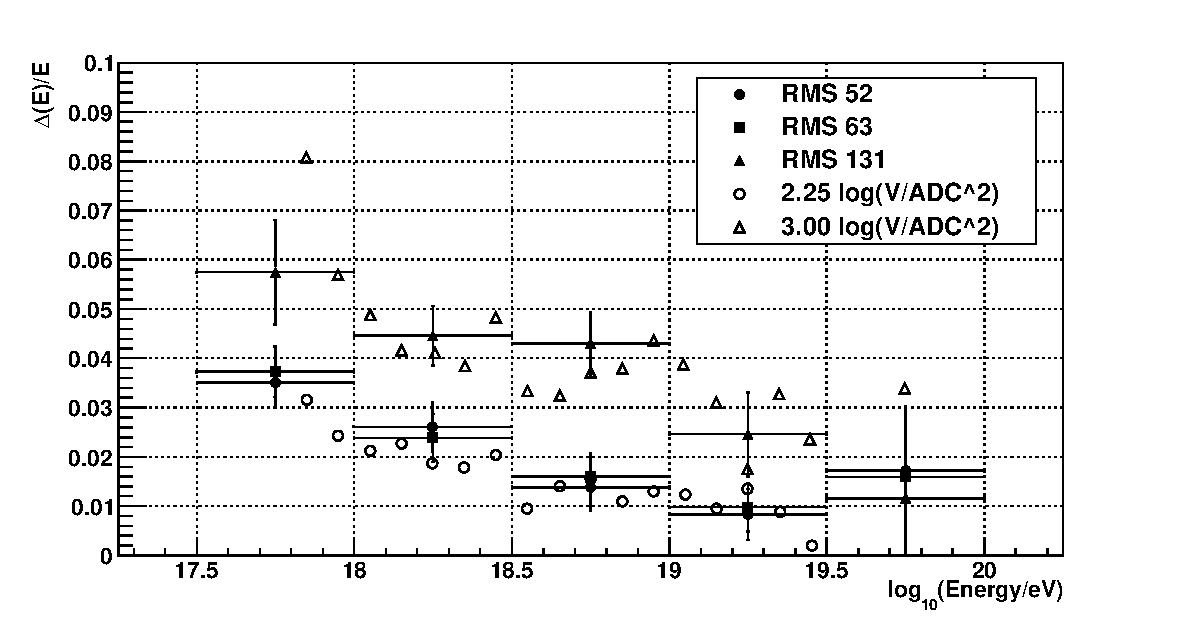
\includegraphics[width=\textwidth]{chapters/graphs/SelectionEff/Smearing_RealData_EnergyBias.pdf}
\caption{Energy Bias using Smearing Method.}
\vspace{3mm}
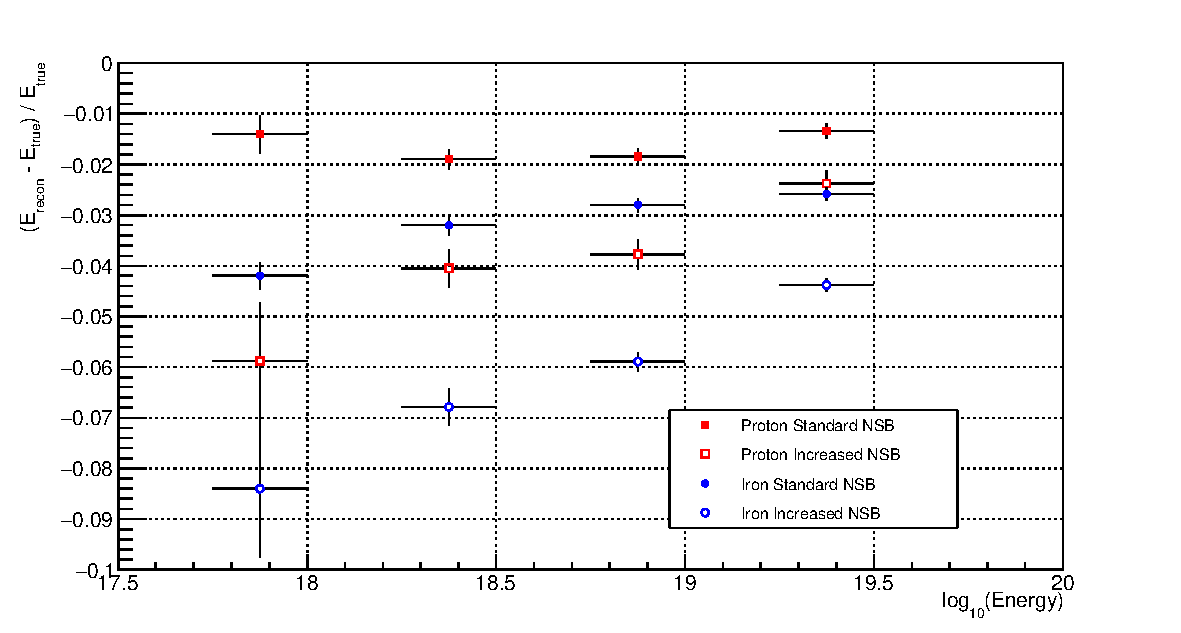
\includegraphics[width=\textwidth]{chapters/graphs/SelectionEff/Simulation_ProtonIron_EnergyBias.pdf}
\caption{Energy Bias using simulated data.}
\end{figure}

\begin{figure}
\centering
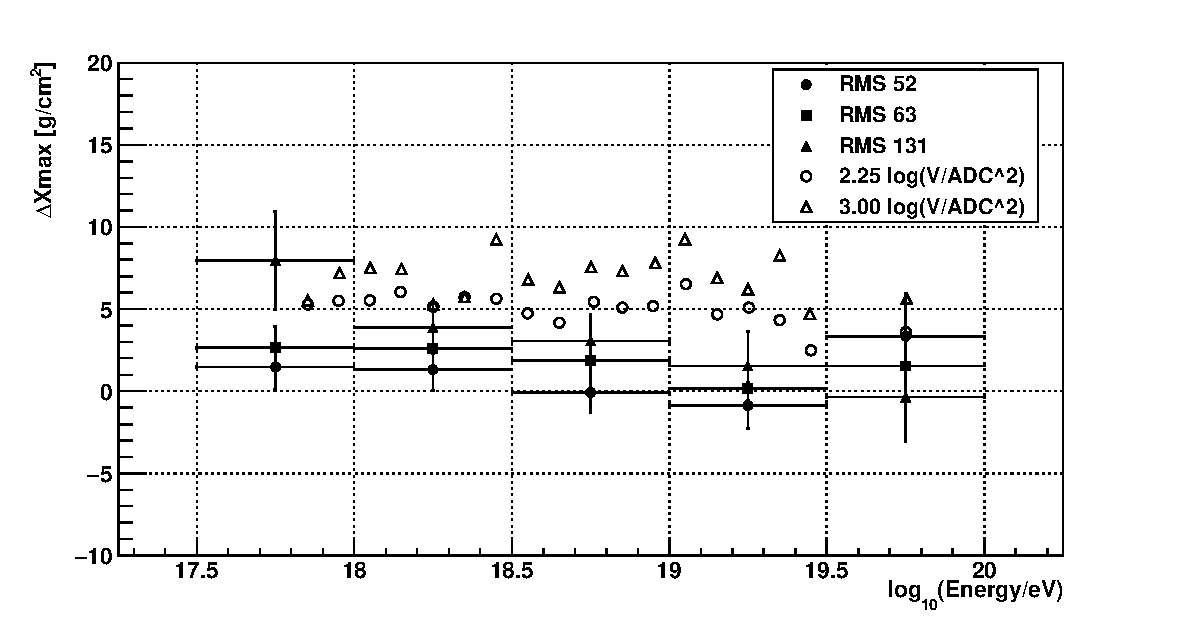
\includegraphics[width=\textwidth]{chapters/graphs/SelectionEff/Smearing_RealData_XmaxBias.pdf}
\caption{Xmax Bias using Smearing Method.}
\vspace{3mm}
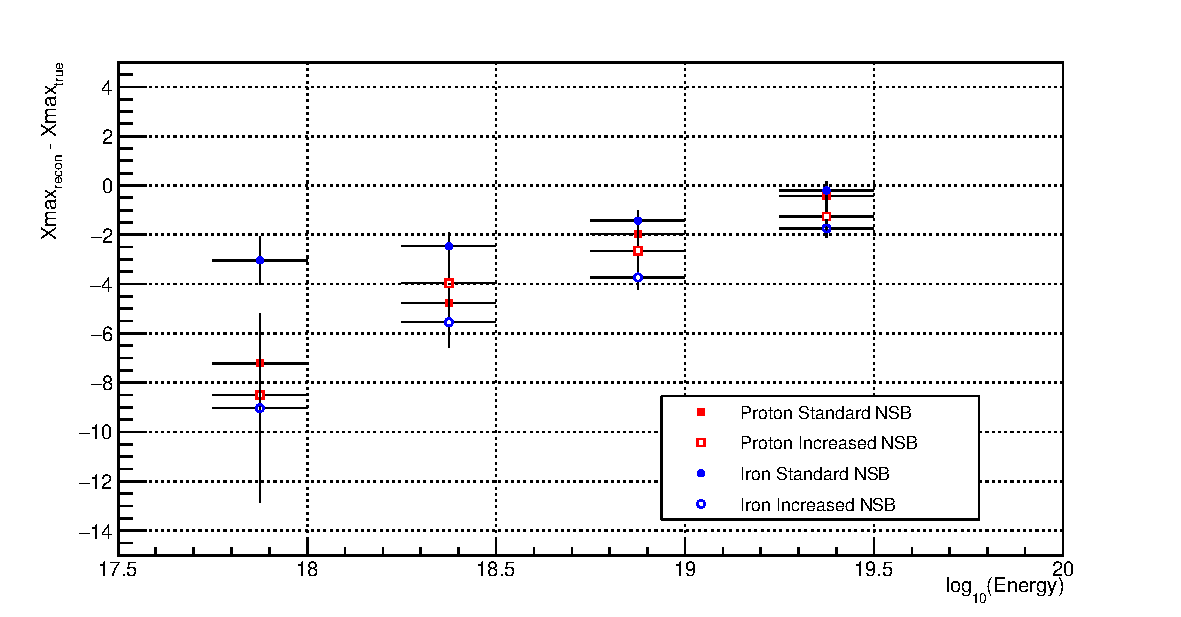
\includegraphics[width=\textwidth]{chapters/graphs/SelectionEff/Simulation_ProtonIron_XmaxBias.pdf}
\caption{Xmax Bias using simulated data.}
\end{figure}

\begin{figure}
\centering
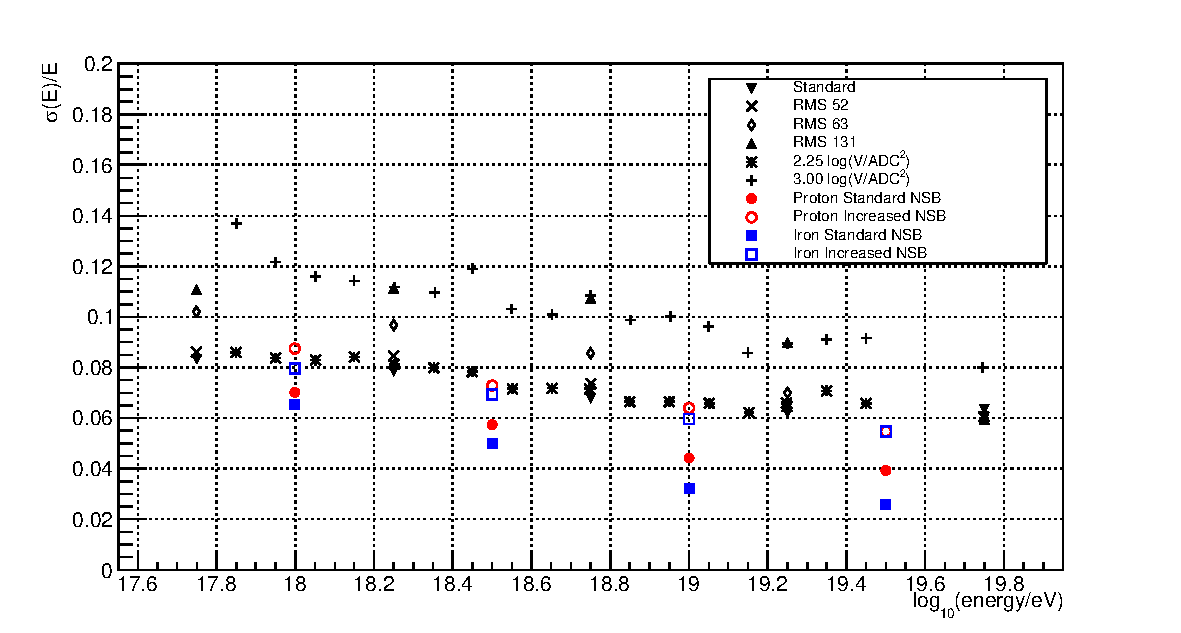
\includegraphics[width=\textwidth]{chapters/graphs/SelectionEff/Combined_EnergyRes_All.pdf}
\caption{Energy Resolution using both Smearing Method data and simulated showers.}
\vspace{3mm}
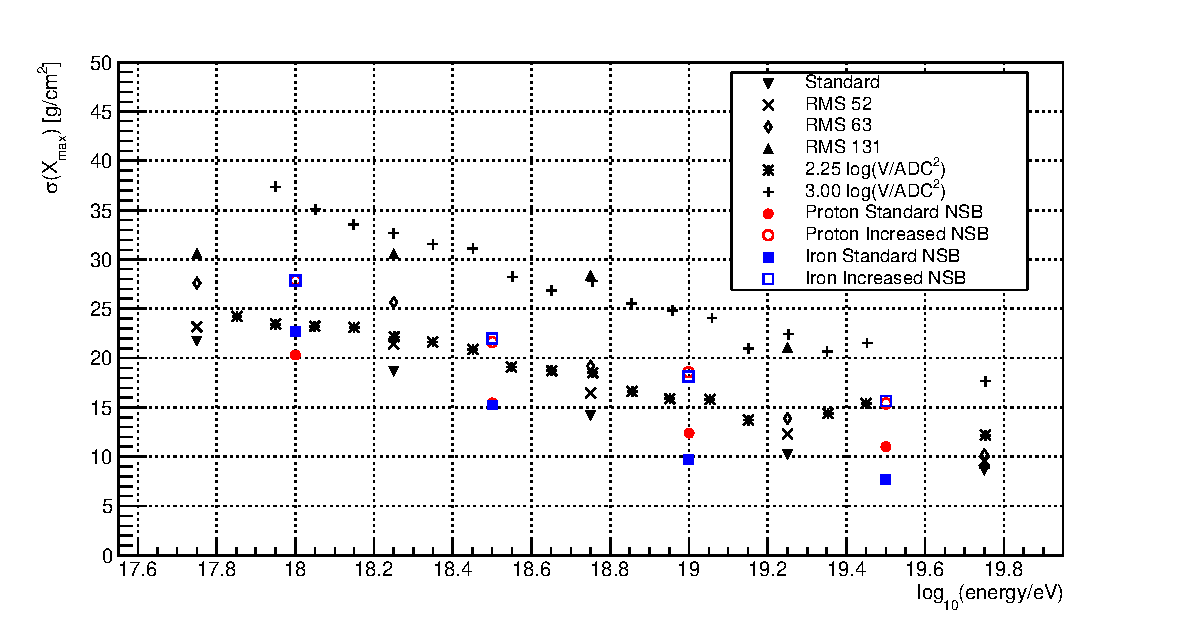
\includegraphics[width=\textwidth]{chapters/graphs/SelectionEff/Combined_XmaxRes_All.pdf}
\caption{Xmax Resolution using both Smearing Method data and simulated showers.}
\end{figure}
